\chapter{Conclusion \& Future Work}

\section{Conclusion}

\begin{figure}[ht!]
    \centering
    \missingfigure[]{Picture of Knee Joint}
    % 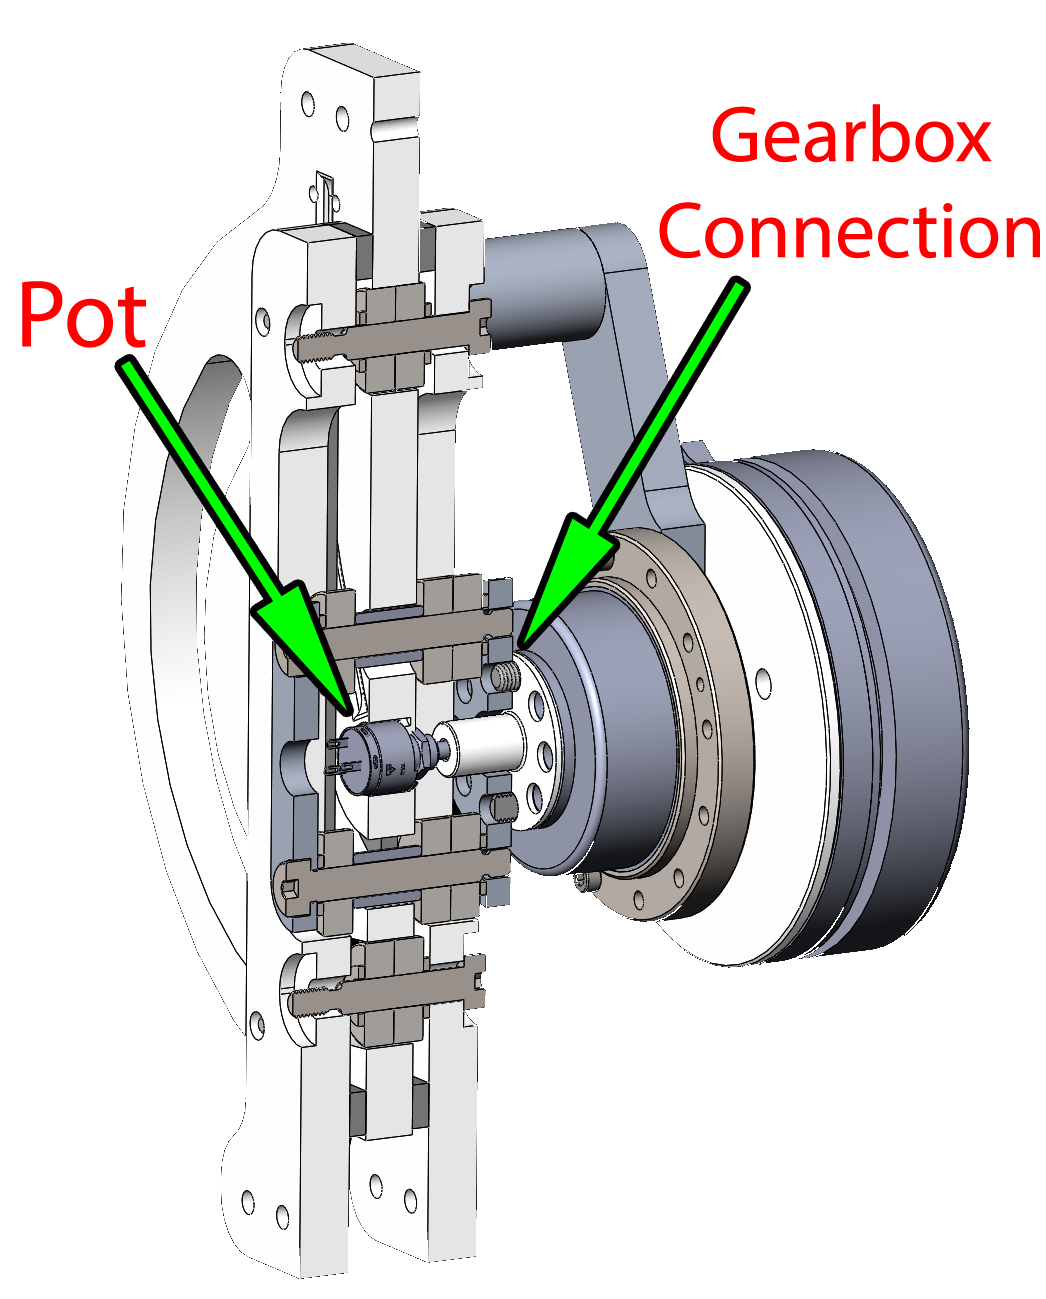
\includegraphics[width=0.7\linewidth]{Figures/Design/KneeJointAssyCrossSection_edit.png}
    \caption{Knee mounted to exoskeleton}
    \label{fig:KneeJointPicture}
\end{figure}

The proposed knee joint developed and tested in this thesis succeeded in all design requirements, even exceeding them in some scenarios. Experimentation showed that the knee could follow a defined tibiofemoral joint trajectory within \(1mm\) of accuracy. The joint itself can also be easily customized to each patient, with only one custom part needing to be machined per person. Integrated sensors allow it to sense joint positioning and report it to the WPI LARRE controllers. Strength analysis demonstrated that the joint can be manufactured from either PLA plastics using a conventional FDM 3D printer or machined out of aluminum. The joint will be able to support the stresses that come from common rehabilitation exercises including sit/stand exercises and walking gait exercises. Finally, the joint will be able to be integrated in the WPI LARRE (Legged Articulated Robotic Rehabilitation Exoskeleton). However, the design proposed is not limited to exoskeletons; the concept of using a cam mechanism to match tibiofemoral relationships can be applied to other orthoses that need to be powered.

\begin{figure}[ht!]
    \centering
    \missingfigure[]{Knee mounted to exoskeleton}
    % 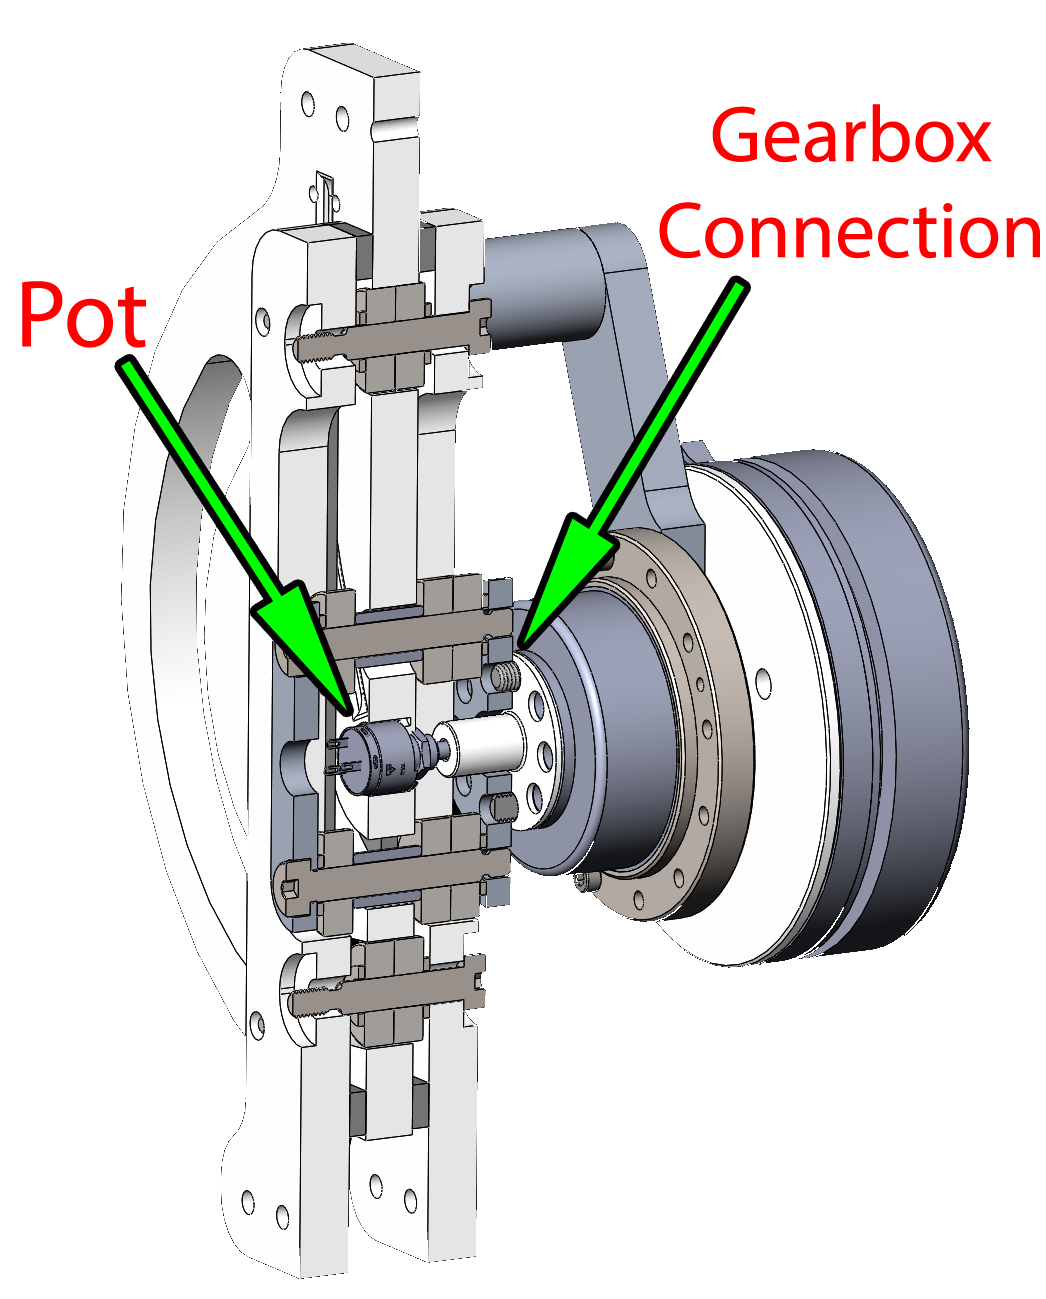
\includegraphics[width=0.7\linewidth]{Figures/Design/KneeJointAssyCrossSection_edit.png}
    \caption{Knee mounted to exoskeleton}
    \label{fig:KneeOnExo}
\end{figure}

\TODO[inline]{Add conclusion for Knee Params}

\section{Future Work}


